\documentclass[cal1spr16Lectures.tex]{subfiles}

\begin{document}

\section[Week 9]{Week 9: 14-18 Mar}

% % %
\subsection[4.1 Maxima and Minima]{\S 4.1 Maxima and Minima}
% % %

% % %
\begin{frame}{\S 4.1 Maxima and Minima}
Chapter 4 is all about applications of the derivative.  In the first couple of sections we examine the graphs of functions and what the derivative can tell us about the graph's behavior and characteristics.
\end{frame}

% % %
\begin{frame}
\small 
\begin{dfn} Let $f$ be defined on an interval $I$ containing $c$.
\begin{itemize}
\item $f$ has an {\bf absolute maximum} value on $I$ at $c$ means $f(c)\ge f(x)$ for every $x$ in $I$.
\item $f$ has an {\bf absolute minimum} value on $I$ at $c$ means $f(c)\le f(x)$ for every $x$ in $I$.
\end{itemize}
\end{dfn}
\end{frame}

% % %
\begin{frame}
\footnotesize
The existence and location of absolute extreme values depend on the function and the interval of interest:
\begin{columns}[T]
\begin{column}{.5\textwidth}
\begin{block}{}
\centering{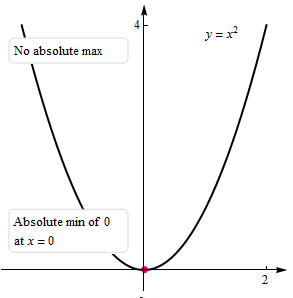
\includegraphics[scale=0.65]{pictures/Fig4_2a}}
\end{block}
\end{column}
\begin{column}{.5\textwidth}
\begin{block}{}
\centering{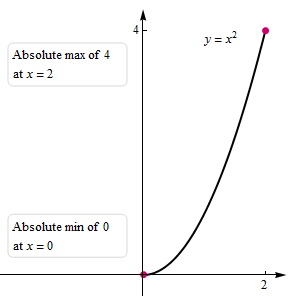
\includegraphics[scale=0.65]{pictures/Fig4_2b}}
\end{block}
\end{column}
\end{columns}
\end{frame}

% % %
\begin{frame}
\frametitle{}
\begin{columns}%[T]
\begin{column}{.5\textwidth}
\begin{block}{}
\centering{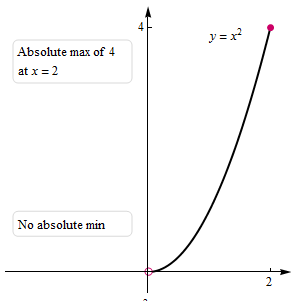
\includegraphics[scale=0.65]{pictures/Fig4_2c}}
\end{block}
\end{column}
\begin{column}{.5\textwidth}
\begin{block}{}
\centering{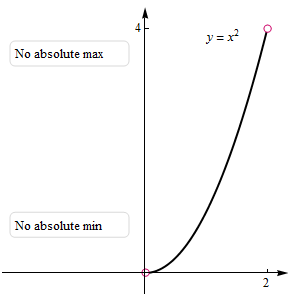
\includegraphics[scale=0.65]{pictures/Fig4_2d}}
\end{block}
\end{column}
\end{columns}
\end{frame}

% % %
\subsubsection{Extreme Value Theorem}
% % % 

% % %
\begin{frame}{\small Extreme Value Theorem}
\small
\begin{thm}[Extreme Value Theorem] A function that is continuous on a closed interval $[a,b]$ has an absolute maximum value and an absolute minimum value on that interval. \end{thm}

\vspace{1pc}
The EVT provides the criteria that ensures absolute extrema:
\begin{itemize}
\item the function must be continuous on the interval of interest;
\item the interval of interest must be closed and bounded.
\end{itemize}
\end{frame}

% % %
\subsubsection{Local Maxima and Minima}
% % %

% % %
\begin{frame}{\small Local Maxima and Minima}
\small
Beyond absolute extrema, a graph may have a number of peaks and dips throughout its interval of interest:
\begin{center}
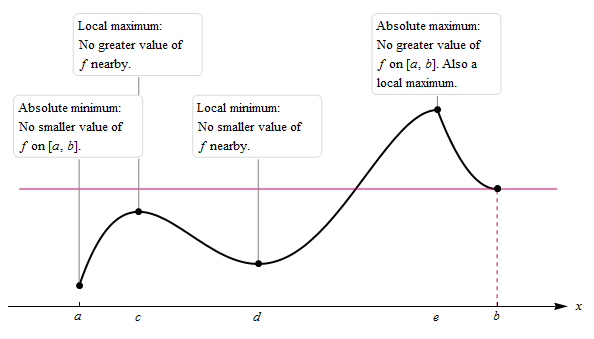
\includegraphics[scale=0.625]{pictures/Fig4_5}
\end{center}
\end{frame}

% % %
\begin{frame}
\frametitle{}
\small
\begin{dfn} Suppose $I$ is an interval on which $f$ is defined and $c$ is an interior point of $I$.
\begin{itemize}
\item If $f(c)\ge f(x)$ for all $x$ in some open interval containing $c$, then $f(c)$ is a {\bf local maximum} value of $f$.
\item If $f(c)\le f(x)$ for all $x$ in some open interval containing $c$, then $f(c)$ is a {\bf local minimum} value of $f$.
\end{itemize}
\end{dfn}
\end{frame}

% % %
\begin{frame}
\frametitle{}
\small
\begin{exe} Use the graph below to identify the points on the interval $[a,b]$ at which local and absolute extreme values occur.
\begin{center}
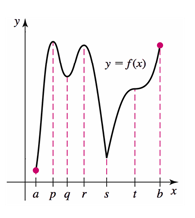
\includegraphics[scale=0.9]{pictures/Ch4Sect1_Prob16}
\end{center}
\end{exe}
\end{frame}

% % %
\subsubsection{Critical Points}
% % %

% % %
\begin{frame}{\small Critical Points}
Based on the previous graph, how is the derivative related to where the local extrema occur?

\vspace{1pc}
Local extrema occur where the derivative either does not exist or is equal to 0.

\begin{dfn} An interior point $c$ of the domain of $f$ at which $f^{\prime}(c)=0$ or $f^{\prime}(c)$ fails to exist is called a {\bf critical point} of $f$. \end{dfn}
\end{frame}

% % %
\subsubsection{Local Extreme Point Theorem}
% % %

% % %
\begin{frame}{\small Local Extreme Point Theorem}
\small
\begin{thm}[Local Extreme Point Theorem] If $f$ has a local minimum or maximum value at $c$ and $f^{\prime}(c)$ exists, then $f^{\prime}(c)=0$.  \alert{\bf (Converse is not true!)} \end{thm}

It is possible for $f^{\prime}(c)=0$ or $f^{\prime}(c)$ not to exist at a point, yet the point not be a local min or max.  Therefore, critical points provide {\bf candidates} for local extrema, but do not guarantee that the points are local extrema (see p.\ 227 immediately before Figure 4.9 for examples).
\end{frame}

% % %
\subsubsection{Locating Absolute Min and Max}
% % %

% % %
\begin{frame}{\small Locating Absolute Min and Max}
%\small
Two facts help us in the search for absolute extrema:

\begin{itemize}
\item Absolute extrema in the interior of an interval are also local extrema, which occur at critical points of $f$.
\item Absolute extrema may occur at the endpoints of $f$.
\end{itemize}
\end{frame}

% % %
\begin{frame}
\frametitle{}
\footnotesize
{\bf Procedure: } Assume that the function $f$ is continuous on $[a,b]$.

\begin{itemize}
\item[1.] Locate the critical points $c$ in $(a,b)$, where $f^{\prime}(c)=0$ or $f^{\prime}(c)$ does not exist.  These points are {\bf candidates} for absolute extrema.
\item[2.] Evaluate $f$ at the critical points and at the endpoints of $[a,b]$.
\item[3.] Choose the largest and smallest values of $f$ from Step 2 for the absolute max and min values, respectively.
\end{itemize}

NOTE:  In this section, given an equation, we can identify critical points and absolute extrema, \alert{BUT NOT LOCAL EXTREMA}.  Techniques for locating local extrema come in later sections.
\end{frame}

% % % 
\begin{frame}
\begin{ex}
On the interval $[-2,2]$, the function $f(x)=x^4$
\begin{itemize}
\item[A. ] has no local or absolute extrema.
\item[B. ] has a local minimum but no absolute minimum.
\item[C. ] has an absolute maximum but no local maxima.
\item[D. ] has an absolute maximum at an interior point of the interval.
\end{itemize}
\end{ex}
\end{frame}

% % %
\begin{frame}%[t]
\frametitle{}
\begin{exe} Given $f(x)=(x+1)^{4/3}$ on $[-8,8]$, determine the critical points and the absolute extreme values of $f$. \end{exe}
\end{frame}

% % %
\subsubsection{Book Problems}

% % %
\begin{frame}
\begin{block}{4.1 Book Problems}
11--35 (odds), 37--49 (odds) 
\end{block}
\end{frame}

% % %
\subsection[4.2 What Derivatives Tell Us]{\S 4.2 What Derivatives Tell Us}
% % %

% % %
\begin{frame}{\S 4.2 What Derivatives Tell Us}
\begin{dfn} Suppose a function $f$ is defined on an interval $I$.
\begin{itemize}
\item We say that $f$ is {\bf increasing} on $I$ if $f(x_2)>f(x_1)$ whenever $x_1$ and $x_2$ are in $I$ and $x_2 > x_1$.
\item We say that $f$ is {\bf decreasing} on $I$ if $f(x_2)<f(x_1)$ whenever $x_1$ and $x_2$ are in $I$ and $x_2 > x_1$.
\end{itemize}
\end{dfn}
\end{frame}

% % %
\subsubsection{How is it related to the derivative?}
% % %

% % %
\begin{frame}{\small How is it related to the derivative?}
%\small
Suppose $f$ is continuous on an interval $I$ and differentiable at every interior point of $I$.

\vspace{1pc}
\begin{itemize}
\item If \alert{$f^{\prime}(x)>0$} for all interior points of $I$, then $f$ is \alert{increasing} on $I$.

\vspace{1pc}
\item If \alert{$f^{\prime}(x)<0$} for all interior points of $I$, then $f$ is \alert{decreasing} on $I$.
\end{itemize}
\end{frame}

% % %
\begin{frame}%[t]
\frametitle{}
\begin{ex} Sketch a function that is continuous on $(-\infty,\infty)$ that has the following properties:

\begin{itemize}
\item $f^{\prime}(-1)$ is undefined;

\vspace{1pc}
\item $f^{\prime}(x)>0$ on $(-\infty,-1)$;

\vspace{1pc}
\item $f^{\prime}(x)<0$ on $(-1,4)$;

\vspace{1pc}
\item $f^{\prime}(x)>0$ on $(4,\infty)$.
\end{itemize}
\end{ex}
\end{frame}

% % %
\begin{frame}%[t]
\frametitle{}
\begin{ex} Find the intervals on which
$$f(x)=3x^3-4x+12$$
is increasing and decreasing.  If you graph $f$ and $f'$ on the same axes, what do you notice?
\end{ex}
\end{frame}

% % %
\subsubsection{First Derivative Test}
% % %

% % %
\begin{frame}{\small First Derivative Test}
\footnotesize
Suppose that $f$ is continuous on an interval that contains a critical point $c$ and assume $f$ is differentiable on an interval containing $c$, except perhaps at $c$ itself.

\begin{itemize}
\item If $f^{\prime}$ \alert{changes sign} from positive to negative as $x$ increases through $c$, then $f$ has a {\bf local maximum} at $c$.

\vspace{0.5pc}
\item If $f^{\prime}$ \alert{changes sign} from negative to positive as $x$ increases through $c$, then $f$ has a {\bf local minimum} at $c$.

\vspace{0.5pc}
\item If $f^{\prime}$ does not change sign at $c$ (from positive to negative or vice versa), then $f$ has {\bf no} local extreme value at $c$.
\end{itemize}

\alert{{\bf NOTE:} The First Derivative Test does NOT test for increasing/decreasing, only local max/min.}  Use it on critical points. 
\end{frame}

% % %
\begin{frame}%[t]
\frametitle{}
\begin{exe} If $f(x)=2x^3+3x^2-12x+1$, identify the critical points on the interval $[-3,4]$, and use the First Derivative Test to locate the local maximum and minimum values.  What are the absolute max and min? \end{exe}
\end{frame}

% % %
\subsubsection{Absolute extremes on any interval}
% % %

% % %
\begin{frame}{\small Absolute extremes on any interval}
\small
The Extreme Value Theorem (cf., Section 4.1) stated that we were guaranteed extreme values \alert{only on closed intervals}.  

\vspace{0.5pc}
\alert{However:}  Suppose $f$ is continuous on an interval $I$ that contains only one local extremum at $(x=)c$.

\begin{itemize}
\item If it is a local minimum, then $f(c)$ \alert{is} the absolute minimum of $f$ on $I$.

\vspace{0.5pc}
\item If it is a local maximum, then $f(c)$ \alert{is} the absolute maximum of $f$ on $I$.
\end{itemize}
\end{frame}

% % %
\subsubsection{Derivative of the derivative tells us:}
% % %

% % %
\begin{frame}{\small Derivative of the derivative tells us:}
\small 
Just as the first derivative $f^{\prime}$ told us whether the function $f$ was increasing or decreasing, the second derivative $f^{\prime\prime}$ also tells us whether $f^{\prime}$ is increasing or decreasing.

\begin{dfn} Let $f$ be differentiable on an open interval $I$.
\begin{itemize}
\item If $f^{\prime}$ is increasing on $I$, then $f$ is {\bf concave up} on $I$.
\item If $f^{\prime}$ is decreasing on $I$, then $f$ is {\bf concave down} on $I$.
\end{itemize}
\end{dfn}

\begin{dfn} If $f$ is continuous at $c$ and $f$ changes concavity at $c$ (from up to down, or vice versa), then $f$ has an {\bf inflection point} at $c$. \end{dfn}
\end{frame}

% % %
\subsubsection{Test for Concavity}
% % % 

% % %
\begin{frame}{\small Test for Concavity}
Suppose that $f^{\prime\prime}$ exists on an interval $I$.

\begin{itemize}
\item If $f^{\prime\prime}>0$ on $I$, then $f$ is \alert{concave up} on $I$.

\vspace{0.5pc}
\item If $f^{\prime\prime}<0$ on $I$, then $f$ is \alert{concave down} on $I$.

\vspace{0.5pc}
\item If $c$ is a point of $I$ at which $f^{\prime\prime}(c)=0$ and $f^{\prime\prime}$ changes signs at $c$, then $f$ has an \alert{inflection point} at $c$.
\end{itemize}
\end{frame}

% % % 
\begin{frame}
\begin{ex}
What would a function with the following properties look like?
\begin{itemize}
\item[1. ] $f'>0$ and $f''>0$
\item[2. ] $f'>0$ and $f''<0$
\item[3. ] $f'<0$ and $f''>0$
\item[4. ] $f'<0$ and $f''<0$ 
\end{itemize}
\end{ex}
\end{frame}

% % %
\subsubsection{Second Derivative Test}
% % %

% % %
\begin{frame}{\small Second Derivative Test}
Suppose that $f^{\prime\prime}$ is continuous on an open interval containing $c$ with $f^{\prime}(c)=0$.

\begin{itemize}
\item If $f^{\prime\prime}(c)>0$, then $f$ has a \alert{local minimum} at $c$.

\vspace{0.5pc}
\item If $f^{\prime\prime}(c)<0$, then $f$ has a \alert{local maximum} at $c$.

\vspace{0.5pc}
\item If $f^{\prime\prime}(c)=0$, then the test is inconclusive.
\end{itemize}

%\vspace{1pc}
%{\bf See the Recap of Derivative Properties (Figure 4.36 on p.\ 242) for a summary.}
\end{frame}

% % % 
\begin{frame}
\begin{exe}
Given $f(x)=2x^3-6x^2-18x$
\begin{itemize}
\item[(a)] Determine the intervals on which it is concave up or concave down, and identify any inflection points.
\item[(b)] Locate the critical points, and use the 2nd Derivative Test to determine whether they correspond to local minima or maxima, or whether the test is inconclusive.
\end{itemize}
\end{exe}
\end{frame}

% % % 
\subsubsection{Book Problems}


% % %
\begin{frame}
\begin{block}{4.2 Book Problems}
11--47 (odds), 53--81 (odds)
\end{block}
\end{frame}

% % %
\subsection[4.3 Graphing Functions]{\S 4.3 Graphing Functions}
% % %

% % %
\begin{frame}{\S 4.3 Graphing Functions}
\footnotesize
{\bf Graphing Guidelines:}
\begin{itemize}
\item[1.] Identify the domain or interval of interest.
\item[2.] Exploit symmetry.
\item[3.] Find the first and second derivatives.
\item[4.] Find critical points and possible inflection points.
\item[5.] Find intervals on which the function is increasing or decreasing, and concave up/down.
\item[6.] Identify extreme values and inflection points.
\item[7.] Locate vertical/horizontal asymptotes and determine end behavior.
\item[8.] Find the intercepts.
\item[9.] Choose an appropriate graphing window and make a graph.
\end{itemize}
\end{frame}

% % %
\begin{frame}
\begin{exe} According to the graphing guidelines, sketch a graph of 
\[f(x)=\frac{x^2}{x^2-4}.\]
\end{exe}
\end{frame}

% % % 
\subsubsection{Book Problems}

% % %
\begin{frame}
\begin{block}{4.3 Book Problems}
7,8, 15-35 (odds), 45-53 
\end{block}
\end{frame}

\end{document}